\chapter{Estado del Arte}
\label{Estado del Arte - YOLO}
% Para el estado del arte
% Debería ser relacionado a object recognition
% Es decir que cosas existen en machine learning para hacer lo que ustedes hacen. ALternativas a YOLO, porque eligimos YOLO, etc
%que modelos me permiten hacer lo mismo que yolo en terminos de funcionalidad
%agregarlos en el estado del arte- basarnos mas nada en la funcionalidad
%nombrar otras alternativas
% buscar benchmarks entre YOLO y otros detectores de objetos

% 1. Benchmarks entre diferentes modelos de detección de objetos y YOLO
% 2. Mejoras incrementales entre las diferentes versiones de YOLO, haciendo hincapié en que beneficio daba cada cosa nueva q se agregaba o modificaba entre versiones. Ej: bag of freebies y bag of specials en YOLOv5.
% 3. Conclusión de la elección


\section{Introducción}
En esta sección se tiene el propósito de hacer una distinción entre los principales tipos Detectores de Objetos. Hacer énfasis en el algoritmo de YOLO y sus variantes. Luego se exponen los Benchmarks (puntos de diferencia) entre los diferentes modelos más populares de detección de objetos y análisis del algoritmo de YOLO. La conclusión de la sección se lleva a cabo con la elección del modelo más conveniente para este proyecto.

\subsection{Detección de Objetos}

Dentro de las arquitecturas Deep Learning se distinguen dos ramas. La primera se conoce como arquitectura de dos fases, generando primero regiones candidatas de la localización del objeto en la imagen y posteriormente clasificando los objetos asignándole una categoría. Se los conoce por detectores de objetos basados en regiones, como los son: Fast R-CNN, Faster R-CNN y R-FCN. Mientras que este tipo de redes son el estado del arte en cuanto a precisión en la localización y clasificación de objetos, tienen la desventaja de ser demasiado lentas para la detección en tiempo real de objetos.

Por otro lado, el segundo tipo de detectores se conocen por tener una arquitectura de una sola fase. Estos realizan una abstracción mayor, donde ven el problema de detección de objetos como un problema de regresión (estimación de las cajas delimitadoras), como lo son SSD y YOLO. Debido a la necesidad de la capacidad de detección de objetos en tiempo real, surgieron las arquitecturas de un paso. Los expertos decidieron reducir el número de fases, logrando en una fase, arquitecturas capaces de inferir directamente a partir de una imagen las coordenadas de las cajas delimitadoras y la verosimilitud por clase. En esta sección, se presentará una de las arquitecturas de un paso usadas
para la detección de objetos en este proyecto.

\subsection{YOLO: You Only Look Once}
   Es uno de los algoritmos de detección de objetos en tiempo real más eficaces, que también abarca varias de las mejores ideas a través de toda la literatura de visión por computadora relacionada con la detección de objetos, por lo que resulta ser un Detector de objetos muy eficaz.
   YOLO \cite{yolo} plantea la detección de objetos como un único problema de regresión, directamente desde los píxeles de la imagen a las coordenadas de la caja delimitadora y a las probabilidades de cada clase, donde una sola red convolucional predice simultáneamente múltiples cajas delimitadoras y probabilidades de clase para esas cajas. YOLO se entrena en imágenes completas y optimiza directamente el rendimiento de la detección. Este modelo unificado tiene varios beneficios sobre los métodos tradicionales de detección de objetos:
   
   \begin{itemize}
        \item YOLO es extremadamente rápido.
            Al enfocar la detección como un problema de regresión, no se necesitan sistemas complejos. Simplemente se ejecuta la red neuronal en una nueva imagen para predecir las detecciones. Además, YOLO alcanza más del doble de la precisión media de otros sistemas en tiempo real.
        \item YOLO trabaja globalmente sobre la imagen. A diferencia de las técnicas de ventana deslizante y propuestas de regiones, YOLO ve toda la imagen durante el tiempo de entrenamiento y prueba, de manera que implícitamente codifica la información contextual sobre las clases, así como su apariencia.
        \item YOLO aprende representaciones generalizables de objetos. Cuando se entrena en imágenes naturales, YOLO es altamente generalizable, es menos probable que se descomponga cuando se aplica a entradas inesperadas por lo que supera los métodos de detección más avanzados
   \end{itemize}
   
   A pesar de estas ventajas, YOLO todavía se queda atrás en cuanto a la precisión con respecto a otros sistemas de detección. Aunque puede identificar rápidamente los objetos en las imágenes, tiene problemas para localizar con precisión algunos objetos, especialmente los pequeños. Esto resultó en un problema para este proyecto, debido a que los objetos de interés aparecen en la mayoría de las imágenes como objetos pequeños.
   
   YOLO \cite{yolo} (Lanzada:8 Junio 2015) ha ido publicando varias versiones, evolucionando desde la versión inicial, cuya estructura podemos ver en la Figura \ref{fig:yolo sistema}, hasta la última de ellas, YOLOv5 \cite{yolov5} - \cite{yolov5} lanzada el 18 Mayo 2020, la cual es una versión modificada de YOLOv4, pasando por las versiones YOLOv2 \cite{yolov2} (25 Diciembre 2016), YOLOv3 \cite{yolov3} (8 Abril 2018) y YOLOv4 \cite{yolov4} (23 Abril 2020).
   
   
\begin{figure}
    \centering
    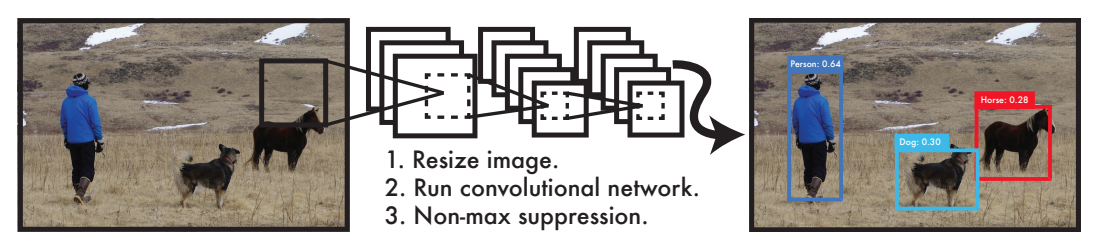
\includegraphics[width=0.9\textwidth]{img/Yolo1sistema.png}
    \caption{El sistema de detección de YOLO: Procesar imágenes con YOLO es simple y directo. El sistema (1) cambia el tamaño de la imagen de entrada a 448 × 448, (2) ejecuta una sola red convolucional en la imagen y (3) establece un umbral para las detecciones resultantes según la confianza del modelo. Fuente: \cite{yolo}}
    \label{fig:yolo sistema}
\end{figure}
   
   
\subsubsection{Funcionamiento de YOLO}

La filosofía de las estructuras YOLO consiste en unificar los diferentes componentes de la detección de objetos en una sola red. El funcionamiento global de la inferencia, se puede ver en la siguiente Figura \ref{fig:yolo funcionamiento}.

\begin{figure}
    \centering
    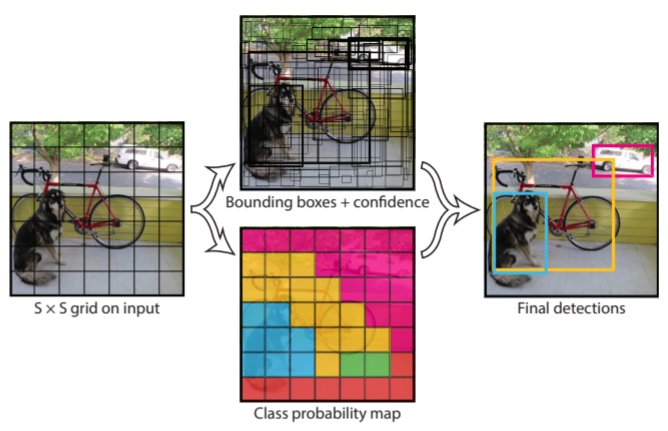
\includegraphics[width=0.9\textwidth]{img/YoloModel.png}
    \caption{Funcionamiento de YOLO: primero se divide la imagen en cuadrículas más pequeñas, sobre éstas se calculan diferentes cajas delimitadoras o bounding boxes y las probabilidades de las distintas clases que se encuentre en ellas, y finalmente se obtienen las detecciones. Fuente: \cite{yolo}. }
    \label{fig:yolo funcionamiento}
\end{figure}

Los componentes principales para formar el algoritmo de detección de objetos YOLO:
    \begin{itemize}
         \item Intersection over Union
         \item Bounding Box Predictions
         \item Non-max suppression
         \item Anchor Boxes
    \end{itemize}

\paragraph{Workflow}
Para llevar a cabo la detección, utilizando YOLO:
\begin{enumerate}
    \item Primero, el algoritmo divide la imagen en una cuadrícula de tamaño SxS celdas (primera imagen de la izquierda Fig.\ref{fig:yolo funcionamiento}). Si el centro de un objeto cae en una celda de la cuadrícula, esa celda es la responsable de detectar el objeto.\\
    \item Cada una de las celdas detecta B posibles “bounding boxes” o cajas delimitadoras y calcula el nivel de certidumbre o confianza (probabilidad de la celda Pc) de cada una de las cajas (imagen del centro), que reflejan que tan seguro está el modelo de que esa caja contiene un objeto y qué tan seguro está de que efectivamente la caja se corresponde al objeto que ha detectado, es decir, se calculan SxSxB diferentes bounding boxes, la gran mayoría de ellas con un Pc muy bajo.
    \[Confianza = P(Objeto) * IOU (truth prediction)\] Si no hay objeto en esa celda, la confianza debería de ser 0, en otro caso debería ser el IOU entre la caja detectada y la leída.\\
    \item Cada una de las cajas delimitadoras está compuesta por 5 predicciones: x, y, w, h y la confianza. Donde (x, y) representa las coordenadas del centro de la caja detectada y (w, h) el ancho y altura respectivamente.\\
    \item Además, cada celda de la cuadrícula también predice C probabilidades condicionales P(Clase \textit{i} $|$ Objeto), una por cada clase, que representan las probabilidades de que en esa celda se encuentre el objeto de la clase \textit{i}. Cabe remarcar, que se predice un vector de C probabilidades condicionales por cada celda, independientemente del número de cajas detectadas B.\\
    \item
    En la inferencia, se multiplican las probabilidades condicionales de cada clase y la confianza de cada caja detectada, obteniendo así las probabilidades específicas de cada clase por cada caja detectada e indicando la probabilidad de que cada clase aparezca en las cajas detectadas y qué tan bien se ajusta dicha caja.
\end{enumerate}


\subsubsection{YOLOv3}

A continuación se hablará de YOLOv3 \cite{yolov3}, que en un principio, fue el modelo elegido para el desarrollar este proyecto como una opción viable de llevarlo a cabo, y con el cual se realizaron las primeras pruebas y evaluaciones de los resultados. \\
Luego se mencionarán brevemente las mejoras que se implementaron en YOLOv3 con respecto a la primera versión YOLO, cuáles mejoras fueron implementadas en YOLOv2 y otras finalmente en YOLOv3.

\paragraph{Mejoras}
\begin{itemize}
    \item Normalización de los lotes en las capas convolucionales.
    \item Clasificador de alta resolución.
    \item Última capa convolucional con anchor boxes o cajas de anclaje, también llamadas cajas a priori. En vez de predecir directamente las cajas, se predicen los offsets con respecto a unas cajas de anclaje previamente predefinidas. Esto es muy útil por que se pueden definir dichas cajas de anclaje para que se adecuen mejor a la forma de los objetos del dataset.
    \item Clusters dimensionales: Como se ha mencionado, en muchos problemas de detección, los objetos tienen una forma determinada, por lo que para calcular las K cajas a priori que mejor cubren esta gama de formas en un dataset, se utiliza el algoritmo KMeans\cite{kmeans}.
    
    \textit{K-means} es un algoritmo de clasificación no supervisada (clusterización), que agrupa objetos en k grupos, basándose en sus características. El agrupamiento se realiza minimizando la suma de distancias entre cada objeto y el centroide de su grupo o cluster. Se suele usar la distancia cuadrática.
    \item Predicción directa de la localización
\end{itemize}

\textbf{Predicción de cajas delimitadoras} \\

Para la predicción de las cajas delimitadoras utiliza la misma metodología que YOLO9000 \cite{yolov2}. La red predice 4 coordenadas para cada anchor boxes \textit{(tx, ty, tw, th)}, de forma que si la celda de la cuadrícula tiene un offset con respecto a la esquina superior izquierda de la imagen de \textit{(cx, xy)} y la caja delimitadora a priori tiene anchura \textit{(pw, ph)}, entonces las predicciones finales son Figura \ref{fig:prediccion de bb}:


\begin{figure}[h!]
    \centering
    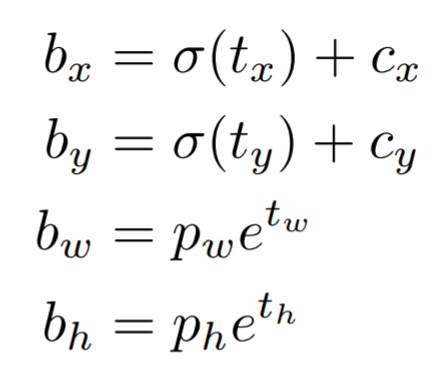
\includegraphics[width=0.25\textwidth]{img/BoundingBoxesFormula.png}
    \caption{Predicciones de las cajas delimitadoras. Fuente: \cite{yolov3}}
    \label{fig:prediccion de bb}
\end{figure}

\newline
En otras palabras, la red predice offsets con respecto a cajas de anclaje (anchor boxes). Se puede ver en la siguiente Figura \ref{fig:cajas delimitdoras} una representación visual de estas ecuaciones. Esto es de mucha utilidad debido a que en muchos problemas de detección, los objetos tienen una forma determinada. Por lo tanto, se definen dichas cajas de anclaje para que se adecuen mejor a la forma de los objetos del dataset. Para calcular las K cajas a priori que mejor cubren esta gama de formas en un dataset, se utiliza el algoritmo K-Means sobre el dataset de entrenamiento.

\begin{figure}
    \centering
    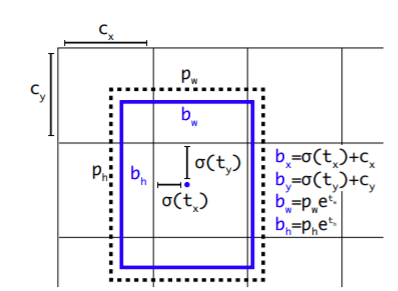
\includegraphics[width=0.7\textwidth]{img/BoundingBoxes.png}\\
    \caption{Cajas delimitadoras con dimensiones previas y predicciones. Se predice el ancho y la altura de la caja como offset desde el centro de la caja. Fuente: \cite{yolov3}}
    \label{fig:cajas delimitdoras}
\end{figure}
\\
Durante el entrenamiento se usa la suma de cuadrados como función de pérdida, de forma que el gradiente viene dado por \[\hat{t} \ast - t\ast \]  donde \[{\hat{t}\ast}\] es el offset predicho por la red y t∗ es el offset real.

\\ \break
YOLOv3 predice una puntuación de objeto para cada caja delimitadora usando regresión logística. Si el cuadro delimitador a priori no es la mejor, pero se superpone a un objeto por encima de un umbral (en este caso 0.5), se ignora la predicción. Es decir, después de obtener todas las predicciones, se procede a eliminar las cajas que estén por debajo de un límite, utilizando una medida que ayude a comparar la precisión de las predicciones del modelo (IoU $>$ 0.5).

A las cajas restantes se les aplica un paso de “non-max suppression”, que sirve para eliminar posibles objetos que fueron detectados por duplicado y así dejar únicamente el más exacto de ellos. \\


\textbf{Predicción de clases} \\

Cada casilla predice las clases que puede contener la caja delimitadora utilizando la clasificación multi-etiqueta, usando para ello, clasificadores logísticos independientes. Durante el entrenamiento se usa como función de pérdida la entropía cruzada binaria. \\


\textbf{Predicciones en diferentes escalas} \\

YOLOv3 realiza predicciones en 3 escalas diferentes. El sistema extrae características de cada una de estas 3 escalas, inspirado y utilizando un concepto similar a las redes piramidales de características o feature pyramid networks \cite{featurepiramid} (en VGG-16) Figura \ref{fig:vgg-16}. En la estructura, después de las capas de extracción de características en YOLOv3 se añaden diferentes capas convolucionales, la última de ellas es la encargada de predecir un vector 3D, codificando las predicciones de cajas delimitadoras, la probabilidad de contener un objeto y predicciones de clase. Así, el vector final es de la forma: \[N * N * (Nboxes ∗ (4 + 1 + Nclasses)\], donde \textit{Nboxes} es el número de cajas predichas en cada escala, \textit{4} se corresponde a los offsets (desplazamiento) de la caja delimitadora, \textit{1} a la predicción del objeto o probabilidad de contener un objeto y \textit{Nclasses} es el número de clases del dataset.

\begin{figure}
    \centering
    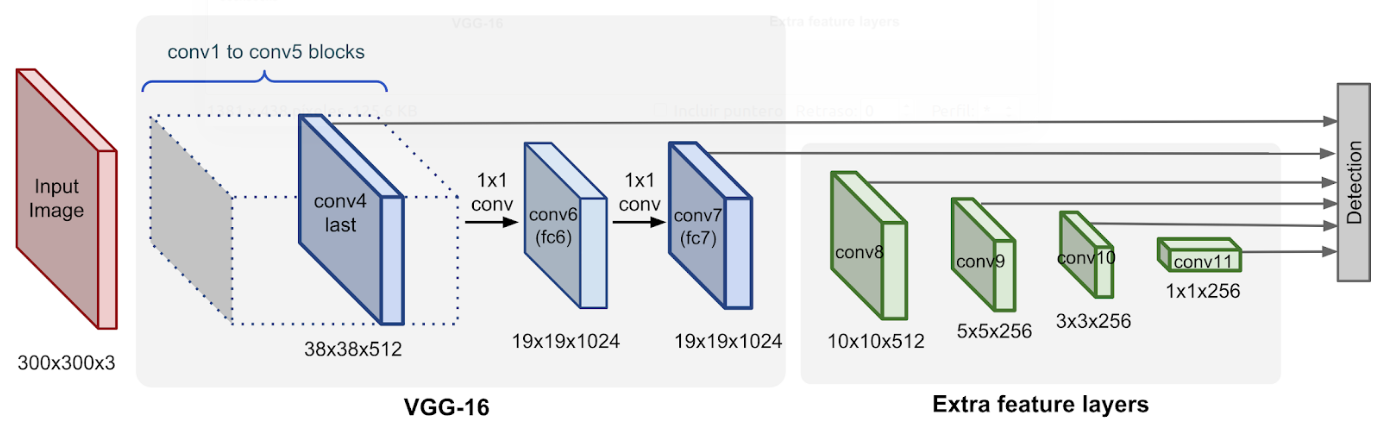
\includegraphics[width=1\textwidth]{img/VGG-16-NetPriamidal.png}
    \caption{Redes Piramidales de Características. Fuente: \cite{10.1007/978-981-19-0011-2_34}}
    \label{fig:vgg-16}
\end{figure}

Se toma el feature map o mapa de características de las dos capas anteriores y se aumenta en 2×. También se toma un mapa de características de las capas anteriores de la red y se fusiona con las características aumentadas de capas subsiguientes, usando concatenación. Este método permite obtener información semántica más significativa. Se realiza el mismo proceso una vez más para predecir cajas para la escala final. Así, las predicciones para la tercera escala se benefician de todos los cálculos previos. De esta manera, se ocupa de muchos más candidatos de bounding boxes de diferentes tamaños. \\


\textbf{Extractor de características} \\

Se utiliza un enfoque híbrido entre el extractor de características utilizado por YOLOv2 (Darknet-19) \cite{yolov2} y capas residuales. Utiliza capas convolucionales sucesivas de 3 × 3 y 1 × 1, con algunas interconexiones o atajos. Tiene 53 capas convolucionales en total y recibe el nombre de Darknet-53. Se puede ver un resumen de su estructura en la Figura \ref{fig:darknet-53}.

\begin{figure}[h!]
    \centering
    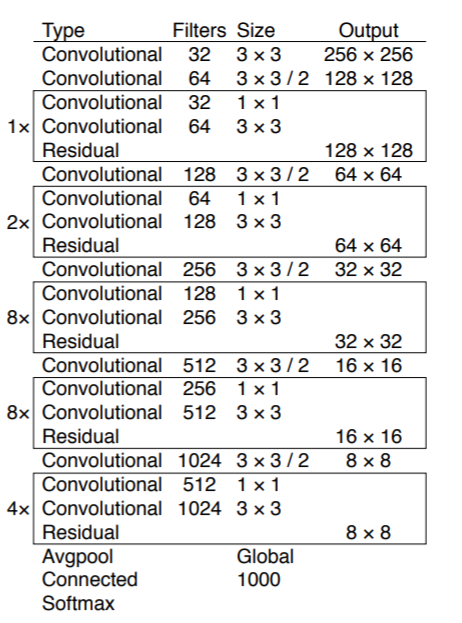
\includegraphics[width=0.6\textwidth]{img/Darknet53.png}
    \caption{Darknet-53. Fuente: \cite{yolov3}}
    \label{fig:darknet-53}
\end{figure}

\newpage
\paragraph{Comparación con otras estructuras}
Se puede ver una comparación en los resultados finales con otras estructuras populares para la detección de objetos en la Figura \ref{fig:comparacion RN}.

\begin{figure} [h!]
    \centering
    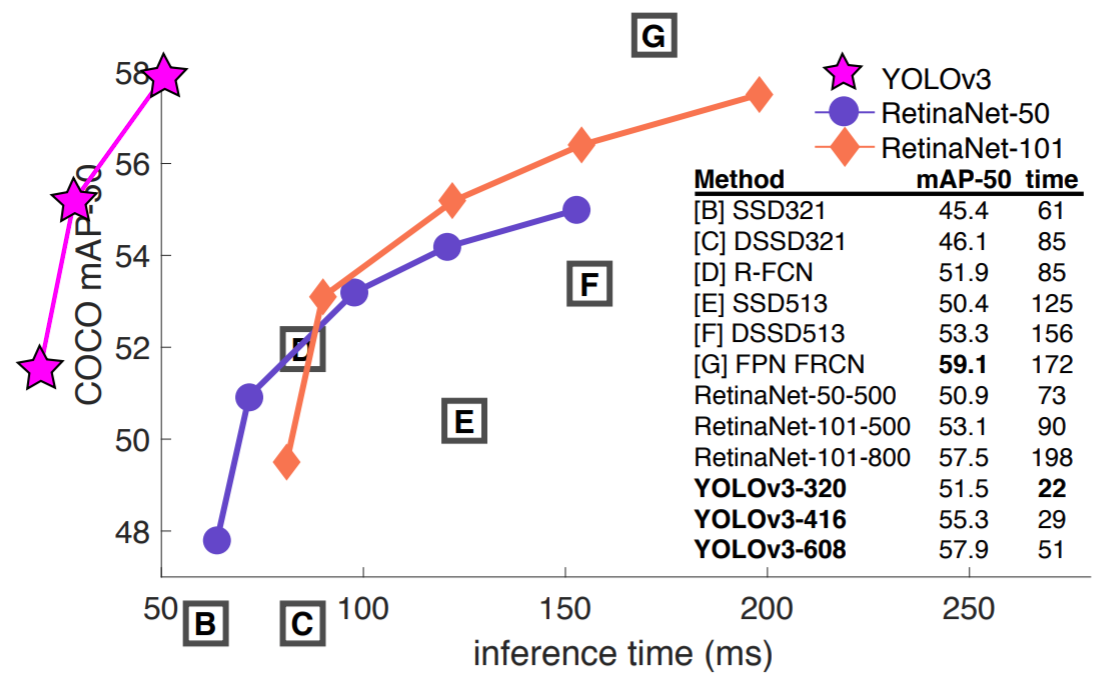
\includegraphics[width=1\textwidth]{img/ComparacionRN.png}
    \caption{Comparación de distintas estructuras de redes neuronales convolucionales: se observa el balance entre velocidad y precisión para 0.5 IOU, destacando YOLOv3 por su gran velocidad y manteniendo una buena precisión. Fuente\cite{yolov3}}
    \label{fig:comparacion RN}
\end{figure}
% 	        \begin{enumerate}
%     			\item Darknet + ResNet como modelo base
%     			\item Regresión Logística para puntaje de confianza
%     			\item Light-weighted base model
%     			\item Predicción multiescala
%     			\item Skip-layer concatenation
% 	        \end{enumerate}
%      
%     \begin{figure}[h]
%     \caption{Yolo - Workflow}
%     \centering
%     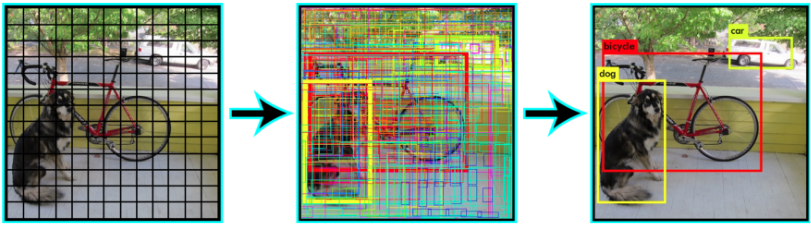
\includegraphics[width=0.95\textwidth]{img/workflowYolo.png}
%     \end{figure}\hfill \break
% 	\subsubsection{Arquitectura de la NN}
% 		4.3.1 Darknet
% 	\subsubsection{YOLO Loss Function}
% 	\subsubsection{YOLOv2}
%         \paragraph{Mejoras}
% 	        \begin{enumerate}
% 			    \item Batch Normalization
% 			    \item Resolucion de Imágenes
% 			    \item Convolutional anchor box detection
% 			    \item K-mean clustering de las dimensiones de las boxes
% 			    \item Predicción de locación directa
% 			    \item Features de granularidad fina
% 			    \item Entrenamiento Multi-escala
% 			    \item Depreciación de softmax para predicción de clase
% 	        \end{enumerate}
% 	\subsubsection{YOLOv3}
%         \paragraph{Mejoras}
% 	        \begin{enumerate}
%     			\item Darknet + ResNet como modelo base
%     			\item Regresión Logística para puntaje de confianza
%     			\item Light-weighted base model
%     			\item Predicción multiescala
%     			\item Skip-layer concatenation
% 	        \end{enumerate}
\newpage
\subsubsection{YOLOv4}

En esta sección se hablará de YOLOv4 \cite{yolov4}, que presenta mejoras considerables con respecto a su predecesor, YOLOv3, tanto en velocidad de inferencia como en precisión de en torno a un 10-12 por ciento, como se observa en la siguiente Figura \ref{fig:object-detection-arqui}.

Además se encuentra una descripción muy detallada junto a los parámetros que utiliza la red en este enlace \cite{yolov4info}. Sin embargo, aunque es una propuesta muy interesante para la detección de objetos en tiempo real por su gran velocidad en cuanto a FPS (Frames per second o Imágenes por segundo) y manteniendo una muy buena precisión con respecto a otros detectores de última generación, al momento de de la selección final del modelo a usar, se opto por la elección de YOLOv5, que es la ultima versión disponible de los YOLO, el cual tiene todas las ventajas de YOLOv4, que se mencionarán brevemente a continuación. 

\paragraph{Mejoras}

\textbf{Nueva Arquitectura} \\

La arquitectura de YOLOv4 se puede dividir en 3 partes:
\begin{enumerate}
    \item {Backbone: Basado en la CSPDarknet53}
    \item {Neck: Basado en SPP y PAN}
    \item {Head: YOLOv3}
\end{enumerate}

\begin{figure}
    \centering
    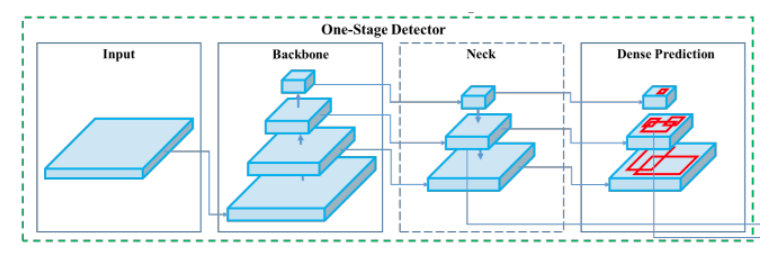
\includegraphics[width=1\textwidth]{img/ObjectDetectionArqui.png}
    \caption{Principales componentes de un Detector de Objetos moderno de una etapa. Fuente: \cite{yolov4}}
    \label{fig:object-detection-arqui}
\end{figure}

Esta nueva arquitectura trae nuevos beneficios con respecto a la versión anterior de YOLO, entre ellas se pueden mencionar que: 
\begin{itemize}
    \item Reduce en gran medida la cantidad de cálculo y mejorar la velocidad de inferencia y la precisión.
    \item Se ocupa de los siguientes tres problemas: Fortalecimiento de la capacidad de aprendizaje de una Red Neuronal Convolucional (CNN).
    Eliminación de cuellos de botella computacionales.
    Reducir los costos de memoria.
    \item Elimina el requerimiento de imagen de entrada de tamaño fijo.
    \item Otorga robustez frente a deformaciones de objetos.
    \item Aumenta el flujo de información propagada a través de la red.
    \item Mejora la predicción de la anchor boxes.
\end{itemize}
\hfill \break

\textbf{Bag of Freebies (BoF)} \\

Bolsa de regalos o Bag of Freebies se denomina al conjunto de técnicas o métodos que cambian la estrategia de entrenamiento o el costo de entrenamiento para mejorar la precisión del modelo. Permiten al detector de objetos ser más preciso sin incrementar el costo computacional, un ejemplo clásico es: data augmentation o el aumento de datos, es un técnica que permite crear variaciones artificiales sobre imágenes del dataset para expandir el conjunto de imágenes existentes y aumenta la capacidad de generalización del modelo.

Para ello se hacen distorsiones fotométricas como: cambiar el brillo, la saturación, el contraste y el ruido o hacer distorsiones geométricas de una imagen, como rotar, recortar, etc. Estas técnicas son un claro ejemplo de un BoF, y ayudan a mejorar la precisión del detector.

\begin{figure}[h!]
    \centering
    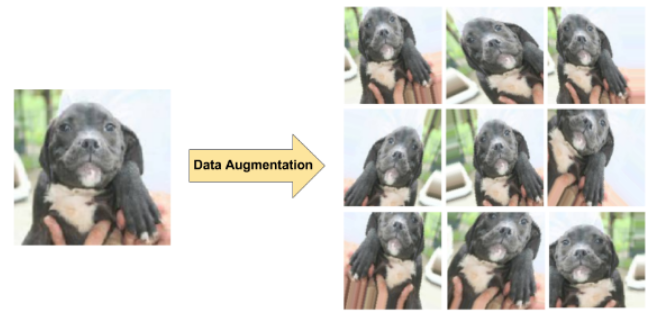
\includegraphics[width=1\textwidth]{img/dataAugmentation.png}
    \caption{Ejemplo de Aumento de datos \cite{dataaug}}
    \label{fig:data-augmentation-ejemplo}
\end{figure}

\begin{enumerate}
    \item {CutMix:}
    En lugar de simplemente eliminar píxeles como en Cutout Figura \ref{fig:cutmix}, se reemplazan las regiones eliminadas con un parche de otra imagen.
    Los parches agregados mejoran la capacidad de localización al requerir que el modelo identifique el objeto desde una vista parcial.
    No quedan píxeles no informativos durante el entrenamiento, lo que hace que el entrenamiento sea más eficiente.

    \begin{figure}[h!]
        \centering
        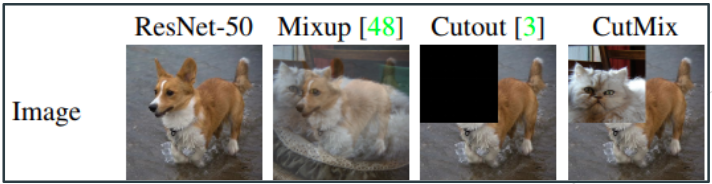
\includegraphics[width=0.9\textwidth]{img/cutMix.png}
        \caption{CutMix}
        \label{fig:cutmix}
    \end{figure}

    \item{Mosaic:}
    Combina 4 imágenes de entrenamiento en una sola, en ciertas proporciones (en lugar de solo dos en CutMix) (Figura \ref{fig:mosaic}).
    Permite que el modelo aprenda a identificar objetos a una escala menor de lo normal y mejorar así la precisión de sus modelos hasta en un 10\%. Combina clases que pueden no verse juntas en su conjunto de entrenamiento.
    
    \begin{figure}[h!]
        \centering
        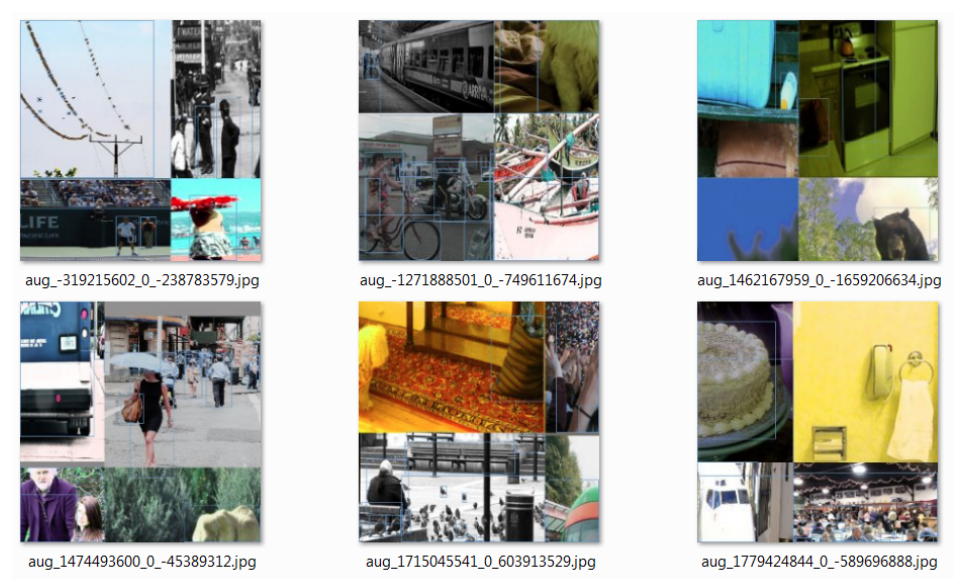
\includegraphics[width=0.8\textwidth]{img/mosaic.png}
        \caption{Mosaic representa un nuevo método de aumento de datos. \cite{yolov4}}
        \label{fig:mosaic}
    \end{figure}
    
    \item{Class label smoothing o Suavizado de etiquetas:}
    Es una técnica de regularización que aborda ambos problemas: overfitting (sobre ajuste) y exceso de confianza.
    Suavizar las etiquetas evita que la red se vuelva demasiado confiada.
    Ayuda al modelo a entrenarse en torno a datos mal etiquetados y, en consecuencia, mejorará su solidez y rendimiento.
    Matemáticamente, se altera el vector \textit{Y} de ground thruth por un factor $\alpha$:
    
    \begin{figure}[h!]
        \centering
        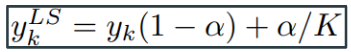
\includegraphics[width=0.4\textwidth]{img/suavizadoEtiqueta.png}
        \label{fig:suavizado-etiqueta}
    \end{figure}
    
    \begin{figure}[h!]
        \centering
        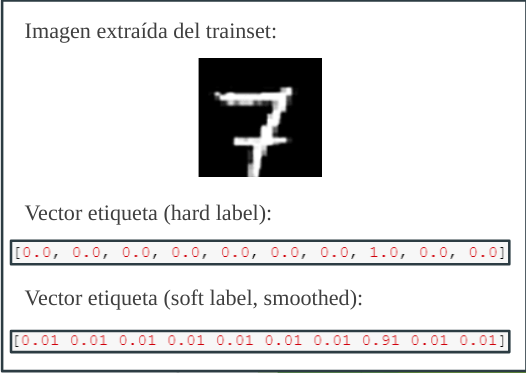
\includegraphics[width=0.8\textwidth]{img/suavizadoEtiquetaVector.png}
        \caption{Suavizado de Etiquetas}
        \label{fig:suavizado-etiqueta-vector}
    \end{figure}
\end{enumerate}
\hfill \break

\textbf{Bag of Specials (BoS)} \\

Como lo mencionan los autores \textit{Bag of Specials} contiene diferentes módulos y módulos de procesamiento posterior que solo aumentan el costo de inferencia en una pequeña cantidad, pero pueden mejorar drásticamente la precisión del detector de objetos. 

Hay muchos módulos diferentes presentes, pero en ésta parte solo se hace foco en uno de éstos métodos selectivos que se muestran en la Figura \ref{fig:bag-of-specials} y se responden el por qué de sus beneficios:

\begin{figure}[h!]
        \centering
        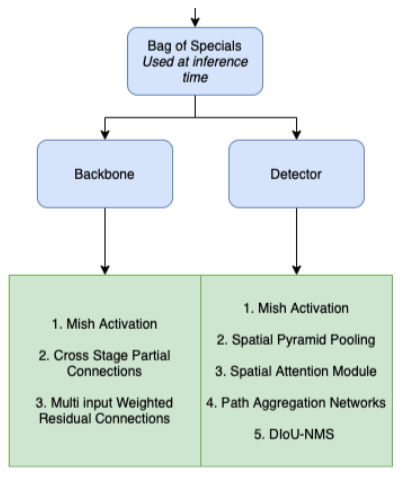
\includegraphics[width=0.8\textwidth]{img/BagOfSpecials.png}
        \caption{Diferentes métodos presentes en la Bag of Specials. Fuente:\cite{img_bag-of-specials}}
        \label{fig:bag-of-specials}
    \end{figure}

\begin{enumerate}
    \item {Módulo de Atención Espacial o Spatial Attention Model (SAM)}

    Se aplica una máscara de atención espacial a las características de entrada, para obtener un features map refinado: Se destacan así las características más relevantes creadas por las capas convolucionales y se remueven las menos importantes. 
    Produciendo una mejora en la clasificación y la detección, con un costo computacional bajo.
    En YOLOv4, una versión modificada de SAM \cite{yolov4} es usada, en la cual no se aplica el maximum ni el average pooling. 
    \\
    
    \begin{figure}[h!]
        \centering
        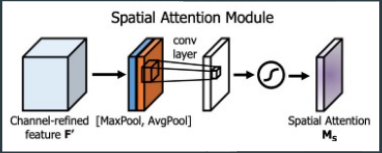
\includegraphics[width=0.8\textwidth]{img/SAM.png}
        \caption{Módulo de Atención Espacial. Fuente: \cite{sam1}}
        \label{fig:sam}
    \end{figure}
\end{enumerate}

    \begin{figure}[h!]
        \centering
        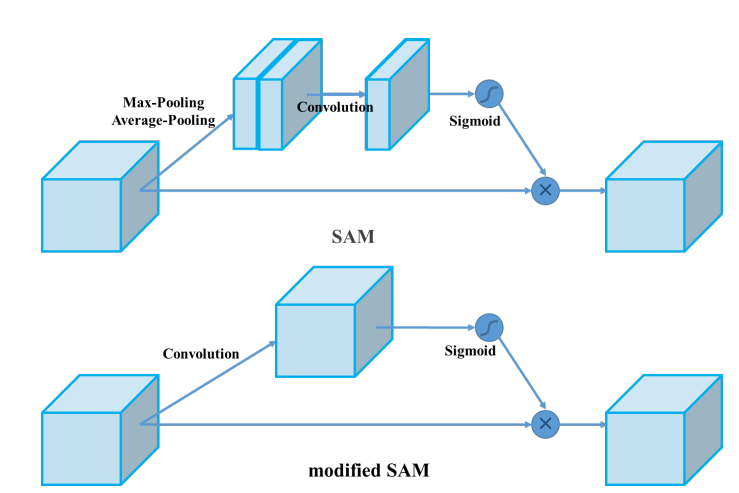
\includegraphics[width=1\textwidth]{img/modifedsam.png}
        \caption{Módulo de Atención Espacial Modificado. Fuente: \cite{yolov4}}
        \label{fig:sam}
    \end{figure}

\subsubsection{YOLOv5}

Poco después del lanzamiento de YOLOv4, se presentó YOLOv5 \cite{yolov5}, aunque sin documentación oficial al día de la redacción de este informe. Sin embargo, se conoce, por medio de foros y repositorios que lo han implementado, que cuenta los las siguientes mejoras:
\paragraph{Mejoras}
     \begin{enumerate}
		\item Es una implementación de YOLOv4 utilizando un framework en Python llamado Pytorch.
		\item Posee muchas optimizaciones algorítmicas y aritméticas.
        \item Se reduce sustancialmente el costo computacional de entrenamiento.
     \end{enumerate}

\paragraph{Memoria y FLOPS}
Cuando se habla de un modelo que es “liviano” se habla de su uso de la \textit{memoria RAM} necesaria para entrenarlo.
La cantidad necesaria viene dada por la cantidad de parámetros que el modelo seleccionado tiene para optimizar.
Si se mantiene constante la arquitectura, a mayor cantidad de parámetros, se suelen obtener mejores predicciones.
Si aumenta la cantidad de parámetros a optimizar, entonces también aumentan la cantidad de operaciones necesarias por iteración, lo que se traduce en mayor uso de CPU+GPU y por ende en tiempo de entrenamiento.
La unidad de medida para estas operaciones se conoce como \textit{FLOPs} (operaciones de punto flotante).\\
\hfill \break

\textbf{Comparación: Memoria y FLOPS} \\

En la siguiente tabla se ve claramente cómo el cambio de arquitectura en YOLO v5l (large), con una cantidad de parámetros incluso menor que YOLOv3, arroja resultados más performantes (mayor FPS) y precisos (mayor AP -precisión promedio-) que éste último.

\begin{figure}[h!]
    \centering
    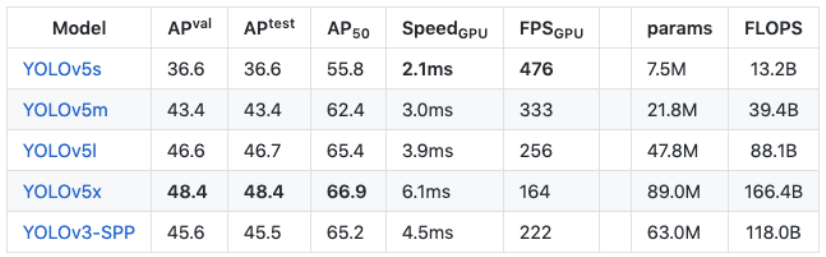
\includegraphics[width=1\textwidth]{img/tablaFLOPS.png}
    \caption{Arquitecturas: Memoria y FLOPS. Fuente: \cite{yolov5}}
    \label{fig:tabla flops}
\end{figure}

\paragraph{Comparación de modelos de YOLOv5}
En la siguiente Figura (\ref{fig:yolo-v5-comparacion}), se puede observar como YOLOv5 hace un excelente rendimiento en la detección de objetos, especialmente el YOLOv5S, con más velocidad.
El objetivo es producir un modelo de detector de objetos que sea muy eficaz (eje Y) en relación con su tiempo de inferencia (eje X). Los resultados preliminares muestran que YOLOv5 lo hace muy bien con éste fin, en comparación con otras técnicas de vanguardia.

\begin{figure}[h!]
    \centering
    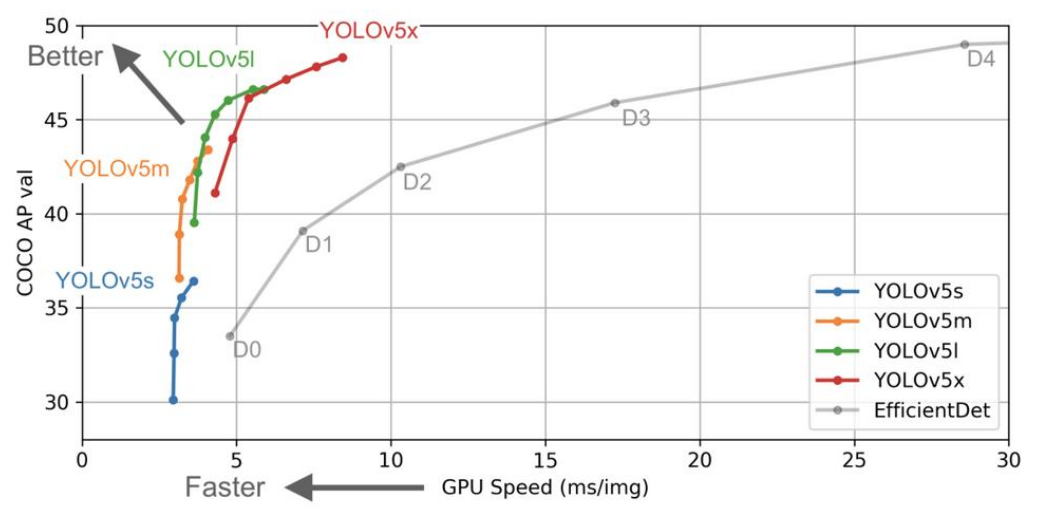
\includegraphics[width=1\textwidth]{img/Yolov5.png}
    \caption{YOLOv5 - Rendimiento. Fuente: \cite{yolov5}}
    \label{fig:yolo-v5-comparacion}
\end{figure}

En resumen, YOLOv5 obtiene la mayor parte de su mejora de rendimiento de los procedimientos de entrenamiento de PyTorch, mientras que la arquitectura del modelo permanece muy cercana a YOLOv4.

\newpage